%------------------------------------------------------------------------------
%Description       : DDMoRe WP7.2.1 First Technical Specification for the Model
%                                   Repository Infrastructure - Introduction 
%Authors           : Mihai Glonț <mglont@ebi.ac.uk>
%                    Camille Laibe <laibe@ebi.ac.uk>
%Organization      : EMBL-EBI
%                    Wellcome Trust Genome Campus
%                    Hinxton
%                    Cambridge
%                    United Kingdom
%------------------------------------------------------------------------------
\section{Introduction}
\label{introduction}
This document describes the technical infrastructure required by the \ddmore Model Repository. The guidelines herein apply not only to the public Repository, but also to any private instances of it.

\subsection{Context}
\label{context}
In a world where inefficient data and knowledge sharing between academia, pharmaceutical companies and regulatory bodies hinders the development of better medicines, the Drug Disease Model Resources project (\ddmore) -- a Europe-wide project funded by Innovative Medicines Initiative Joint Undertaking -- seeks to create an environment governed by standards that addresses these shortcomings. Specifically, the \ddmore consortium is developing a common definition language for data, models and work flows, as well as a standard for storing and exchanging \glspl{model} and associated metadata\cite{ddmore:dow}.

The main focus on this specification is the objective of Task 7.2: the \ddmore Model Repository. It aims to provide a central repository for the models created by the project, allowing their share and encouraging their reuse. The Repository is closely linked with other deliverables of \ddmore. For instance, the pre-competitive models that will populate the Model Repository initially will be provided by WP1. The models will be encoded in the XML-based format developed by WP4, and the Repository will rely on the software library created by the Task 2.3 in order to manipulate the models. Finally, the published models stored in the \ddmore Model Repository will be showcased in the Public Instance of the Modelling Framework, generated by Task 7.1.


\subsection{Objectives}
\label{objectives}
The main objectives of the Repository are to provide:
\begin{itemize}
  \item a central, versioned, storage place for public and private models
  \item a way to display individual models
  \item a way to search for models
  \item a way to download models
  \item various means to access to the stored models (for both users and tools)
\end{itemize}

The interactions between users, the Model Repository and other components of the project (such as the interoperability framework) are depicted in Figure~\ref{fig:userInteraction}. As such, one may access the Repository directly -- through the web-based user interface -- or indirectly, via the Modelling Interoperability Framework, that uses the Task Execution Language (TEL) and the software library created in WP2.3 to access and store models in the \ddmore Model Repository.


\subsection{Type of users}
\label{users}
The different type of users of the system are:
\begin{description}
  \item[Visitor] an anonymous user accessing published models.
  \item[Owner] the user who submitted the model and has ultimate ownership of what is done to it and how and
when it is published.
  \item[Editor] any user who is able to modify and add information to an existing unpublished or published model. Typically the Owner of a model is
also an Editor of this model.
  \item[Collaborator] any user who is able to access an unpublished model.
  \item[Reviewer] a user who can access an unpublished model. This role can be limited in time.
  \item[Administrator] a user who is responsible for the security, management and maintenance of the system.
\end{description}

\textbf{TODO resize images externally and drop the need to scale them in \LaTeX}

\begin{figure}[h!]
\centering
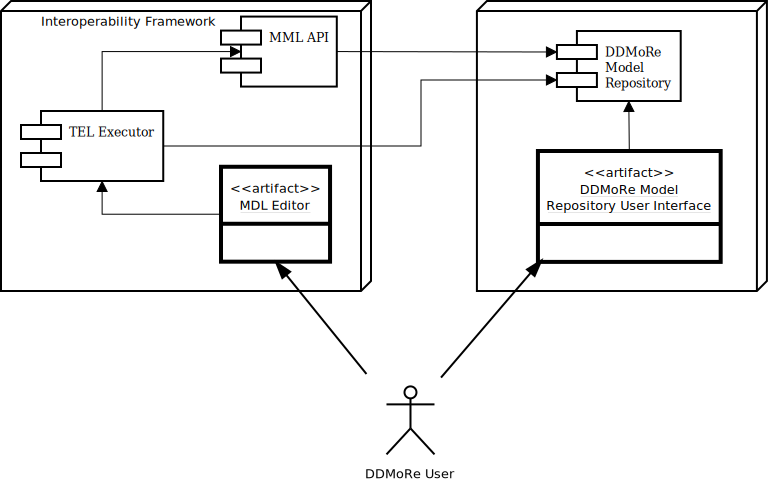
\includegraphics[width=0.75\linewidth]{img/UserInteraction}
\caption{Interactions between users, the interoperability framework and the Model Repository.}
\label{fig:userInteraction}
\end{figure}


